% This line sets the project root file.
% !TEX root = Notes_Gauging_Defects.tex
% !TEX spellcheck = en_US

\subsection{Example: $\Vec(\Z/2\Z)$ spin chain}
\label{subsec:VecZ2}

We consider a one-dimensional spin chain of $N$ particles, where each particle can be in the spin-up state or in the spin-down state, i.e., a chain
	\begin{figure}[H]
		
\begin{tikzpicture}[scale=1.5]
			\fill[black] (0,0) circle (0.07cm);
			\fill[black] (0.5,0) circle (0.07cm);
			\fill[black] (1,0) circle (0.07cm);
			\fill[black] (1.5,0) circle (0.07cm);
			\fill[black] (2,0) circle (0.07cm);
			\fill[black] (2.5,0) circle (0.07cm);
			\fill[black] (3,0) circle (0.07cm);
			\fill[black] (4,0) circle (0.07cm);
			\node at (3.5,0) {$\dots$};
		\end{tikzpicture}
	\end{figure}
\noindent
whose Hilbert space is 
	\begin{equation}
		\mathcal{H}_0=\bigotimes_{i=1}^N \mathbb{C}^2.
	\end{equation}
We now introduce defects, which means that one of the spins, say the spin at site $j$, is replaced by a different kind of spin, e.g., no spin (indicated in red): 
	\begin{figure}[H]
		
\begin{tikzpicture}[scale=1.5]
			\fill[black] (0,0) circle (0.07cm);
			\fill[black] (0.5,0) circle (0.07cm);
			\fill[black] (1,0) circle (0.07cm);
			\fill[black] (1.5,0) circle (0.07cm);
			\fill[red] (2,0) circle (0.07cm);
			\fill[black] (2.5,0) circle (0.07cm);
			\fill[black] (3,0) circle (0.07cm);
			\fill[black] (4,0) circle (0.07cm);
			\node at (3.5,0) {$\dots$};
		\end{tikzpicture}
	\end{figure}
\noindent
This corresponds to replacing the Hilbert space $\mathbb{C}^2$ at site $j$ with $\mathbb{C}$, which results in the overall Hilbert space
	\begin{equation}
		\mathcal{H}_1^{(j)}=\left(\bigotimes_{i=1}^{j-1}\mathbb{C}^2\right)\otimes\mathbb{C}\otimes\left(\bigotimes_{i=j+1}^N\mathbb{C}^2\right).
	\end{equation}
The subscript here denotes the number of defects in the chain and the superscript indicates at which site the defect appears. If we want to consider both possibilities, having no defect and having a defect at site $j$, we use the Hilbert space
	\begin{equation}
		\mathcal{H}=\mathcal{H}_0\oplus\mathcal{H}_1^{(j)}.
	\end{equation}
We can also allow the defect to move, which means we still restrict the setting to only one defect in total, but it can happen at any site. Hence, the overall Hilbert space becomes
	\begin{equation}
		\mathcal{H}=\mathcal{H}_0\oplus\left(\bigoplus_{j=1}^N\mathcal{H}_1^{(j)}\right).
	\end{equation}
This construction can be generalized to an arbitrary number of defects: The Hilbert space for having defects two defects in the chain, say at sites $j$ and $k$, is 
	\begin{equation}
		\mathcal{H}_2^{(j,k)}=\left(\bigotimes_{i=1}^{j-1}\mathbb{C}^2\right)\otimes\mathbb{C}\otimes\left(\bigotimes_{i=j+1}^{k-1}\mathbb{C}^2\right)\otimes\mathbb{C}\otimes\left(\bigotimes_{i=k+1}^{N}\mathbb{C}^2\right).
	\end{equation}
Again, if we allow these defects to move and also include the possibilities of having only one defect and no defect at all, the overall Hilbert space is
	\begin{equation}
		\mathcal{H}=\mathcal{H}_0\oplus\left(\bigoplus_{j=1}^N\mathcal{H}_1^{(j)}\right)\oplus\left(\bigoplus_{j=1}^N\bigoplus_{k\neq j}\mathcal{H}_2^{(j,k)}\right).
	\end{equation}
We can continue this construction until we have a defect at every site of the chain, i.e.
	\begin{equation}
		\mathcal{H}_N=\bigotimes_{i=1}^N\mathbb{C},
	\end{equation}
and the overall Hilbert space is then
	\begin{equation}
		\mathcal{H}=\bigoplus_{n\in\#\mathrm{defects}}\mathcal{H}_n,
	\end{equation}
where $\mathcal{H}_n$ is the direct sum of all possible Hilbert spaces with $n$ defects, as constructed above. Since this is now a very complicated Hilbert space, we can also think about it in a different and simpler way: at each site, the particle can be in one of three states: spin up, spin down, or no spin. Hence, we have effectively a three-level system at each site of the chain, and therefore the overall Hilbert space can be written as
	\begin{equation}
		\mathcal{H}\cong\bigotimes_{j=1}^N\left(\mathbb{C}\oplus\mathbb{C}^2\right).
	\end{equation}

We will now look at the example of a particle chain with $\Vec(\Z/2\Z)$ fusion rules, i.e.\ the objects are either $0$ or $1$ and the fusion is given by addition $\mathrm{mod}\ 2$. We consider the following chain:
	\begin{figure}[H]
		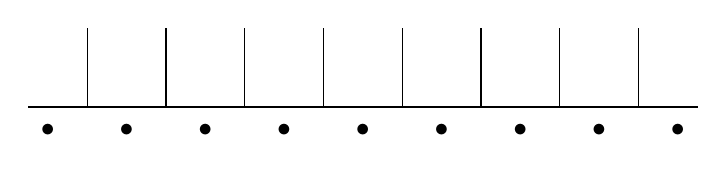
\begin{tikzpicture}
			\draw (-0.25,0) -- (8.25,0);
			\draw (0.5,0) -- (0.5,1);
			\draw (1.5,0) -- (1.5,1);
			\draw (2.5,0) -- (2.5,1);
			\draw (3.5,0) -- (3.5,1);
			\draw (4.5,0) -- (4.5,1);
			\draw (5.5,0) -- (5.5,1);
			\draw (6.5,0) -- (6.5,1);
			\draw (7.5,0) -- (7.5,1);
			\node at (0,-0.3) {$\bullet$};
			\node at (1,-0.3) {$\bullet$};
			\node at (2,-0.3) {$\bullet$};
			\node at (3,-0.3) {$\bullet$};
			\node at (4,-0.3) {$\bullet$};
			\node at (5,-0.3) {$\bullet$};
			\node at (6,-0.3) {$\bullet$};
			\node at (7,-0.3) {$\bullet$};
			\node at (8,-0.3) {$\bullet$};
		\end{tikzpicture}
	\end{figure}
\noindent
where the vertical lines are fixed and the bullets can either be $0$ or $1$ (according to the fusion rules), hence each bullet represents the space $\mathbb{C}^2$.
If we, for instance, only fuse $1$-particles to the chain, the value of the bullets is fixed by the fusion rules: When we fix the boundary labels (e.g., to $1$), the only possible labelling is
	\begin{figure}[H]
		\begin{tikzpicture}
			\draw (-0.25,0) -- (8.25,0);
			\draw (0.5,0) -- (0.5,1);
			\draw (1.5,0) -- (1.5,1);
			\draw (2.5,0) -- (2.5,1);
			\draw (3.5,0) -- (3.5,1);
			\draw (4.5,0) -- (4.5,1);
			\draw (5.5,0) -- (5.5,1);
			\draw (6.5,0) -- (6.5,1);
			\draw (7.5,0) -- (7.5,1);
			\node at (0.5,1.3) {$1$};
			\node at (1.5,1.3) {$1$};
			\node at (2.5,1.3) {$1$};
			\node at (3.5,1.3) {$1$};
			\node at (4.5,1.3) {$1$};
			\node at (5.5,1.3) {$1$};
			\node at (6.5,1.3) {$1$};
			\node at (7.5,1.3) {$1$};
			\node at (0,-0.3) {$1$};
			\node at (1,-0.3) {$0$};
			\node at (2,-0.3) {$1$};
			\node at (3,-0.3) {$0$};
			\node at (4,-0.3) {$1$};
			\node at (5,-0.3) {$0$};
			\node at (6,-0.3) {$1$};
			\node at (7,-0.3) {$0$};
			\node at (8,-0.3) {$1$};
		\end{tikzpicture}
	\end{figure}
\noindent
Hence, we have a unique ground state and the only vertices occurring in this case are
	\begin{figure}[H]	
		\begin{tikzpicture}
			\draw (0,0) -- (1.5,0);
			\draw (0.75,0) -- (0.75,1);
			\node at (0,-0.3) {$0$};
			\node at (1.5,-0.3) {$1$};
			\node at (0.75,1.3) {$1$};
		\end{tikzpicture}
		\hspace{20pt}
		\begin{tikzpicture}
			\draw (0,0) -- (1.5,0);
			\draw (0.75,0) -- (0.75,1);
			\node at (0,-0.3) {$1$};
			\node at (1.5,-0.3) {$0$};
			\node at (0.75,1.3) {$1$};
		\end{tikzpicture}
	\end{figure}
\noindent
Analogously, if we only allow $0$s to fuse to the chain, and the outer labels are fixed to $1$, the only possible labeling is 
	\begin{figure}[H]
		\begin{tikzpicture}
		\draw (-0.25,0) -- (8.25,0);
		\draw (0.5,0) -- (0.5,1);
		\draw (1.5,0) -- (1.5,1);
		\draw (2.5,0) -- (2.5,1);
		\draw (3.5,0) -- (3.5,1);
		\draw (4.5,0) -- (4.5,1);
		\draw (5.5,0) -- (5.5,1);
		\draw (6.5,0) -- (6.5,1);
		\draw (7.5,0) -- (7.5,1);
		\node at (0.5,1.3) {$0$};
		\node at (1.5,1.3) {$0$};
		\node at (2.5,1.3) {$0$};
		\node at (3.5,1.3) {$0$};
		\node at (4.5,1.3) {$0$};
		\node at (5.5,1.3) {$0$};
		\node at (6.5,1.3) {$0$};
		\node at (7.5,1.3) {$0$};
		\node at (0,-0.3) {$1$};
		\node at (1,-0.3) {$1$};
		\node at (2,-0.3) {$1$};
		\node at (3,-0.3) {$1$};
		\node at (4,-0.3) {$1$};
		\node at (5,-0.3) {$1$};
		\node at (6,-0.3) {$1$};
		\node at (7,-0.3) {$1$};
		\node at (8,-0.3) {$1$};
		\end{tikzpicture}
	\end{figure}
	\noindent
If we had fixed the outer labels to $0$, all bullets would have to be $0$. Hence, the only vertices occurring in these cases are
	\begin{figure}[H]	
		\begin{tikzpicture}
		\draw (0,0) -- (1.5,0);
		\draw (0.75,0) -- (0.75,1);
		\node at (0,-0.3) {$0$};
		\node at (1.5,-0.3) {$0$};
		\node at (0.75,1.3) {$0$};
		\end{tikzpicture}
		\hspace{20pt}
		\begin{tikzpicture}
		\draw (0,0) -- (1.5,0);
		\draw (0.75,0) -- (0.75,1);
		\node at (0,-0.3) {$1$};
		\node at (1.5,-0.3) {$1$};
		\node at (0.75,1.3) {$0$};
		\end{tikzpicture}
	\end{figure}
\noindent
This means that in the case of open boundary conditions, the chain has a \emph{unique ground state} once we fix the outer labels of the chain. The situation is different for periodic boundary conditions: since the only requirement here is that the label at site $n+1$ has to equal the label at site $1$, there are always two possibilities of labeling the chain. For instance, in the case of only fusing $1$s to the chain, the two possibilities are
	\begin{figure}[H]
		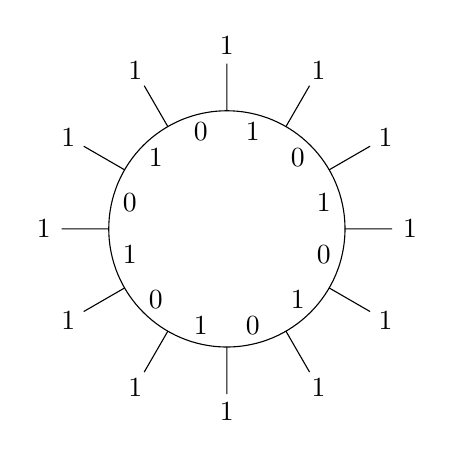
\begin{tikzpicture}[scale=1.5]
			\def\Radius{1cm}
			\draw (0,0) circle[radius=\Radius];
			\draw
			\foreach \a in {0, 30, ..., 330} {
				(\a:\Radius) -- (\a:1.4)
			};
			\foreach \a in {0, 30, ..., 330} {
				\node at (\a:1.55) {$1$};
			};
			\foreach \a in {45, 105, ..., 375} {
				\node at (\a:0.85) {$0$};
			};
			\foreach \a in {15, 75, ..., 315} {
				\node at (\a:0.85) {$1$};
			};
		\end{tikzpicture}
		\hspace{40pt}
		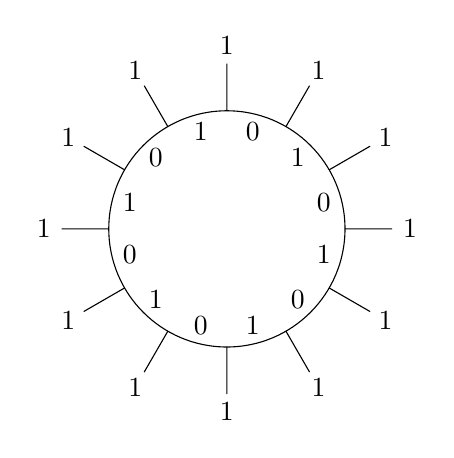
\begin{tikzpicture}[scale=1.5]
			\def\Radius{1cm}
			\draw (0,0) circle[radius=\Radius];
			\draw
			\foreach \a in {0, 30, ..., 330} {
				(\a:\Radius) -- (\a:1.4)
			};
			\foreach \a in {0, 30, ..., 330} {
				\node at (\a:1.55) {$1$};
			};
			\foreach \a in {45, 105, ..., 375} {
				\node at (\a:0.85) {$1$};
			};
			\foreach \a in {15, 75, ..., 315} {
				\node at (\a:0.85) {$0$};
			};
		\end{tikzpicture}
	\end{figure}
\noindent
In case of fusing $0$ to the chain, we can either allow only $0$s or only $1$ as labels of the chain. Therefore, the chain with periodic boundary conditions has two ground states, hence it represents a qubit.

We will now introduce defects to this model, indicated by red lines that fuse to the chain, e.g.\ a chain with one defect would be
	\begin{figure}[H]
		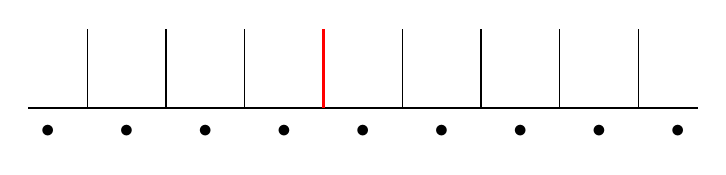
\begin{tikzpicture}
		\draw (-0.25,0) -- (8.25,0);
		\draw (0.5,0) -- (0.5,1);
		\draw (1.5,0) -- (1.5,1);
		\draw (2.5,0) -- (2.5,1);
		\draw[red,line width=0.4mm] (3.5,0) -- (3.5,1);
		\draw (4.5,0) -- (4.5,1);
		\draw (5.5,0) -- (5.5,1);
		\draw (6.5,0) -- (6.5,1);
		\draw (7.5,0) -- (7.5,1);
		\node at (0,-0.3) {$\bullet$};
		\node at (1,-0.3) {$\bullet$};
		\node at (2,-0.3) {$\bullet$};
		\node at (3,-0.3) {$\bullet$};
		\node at (4,-0.3) {$\bullet$};
		\node at (5,-0.3) {$\bullet$};
		\node at (6,-0.3) {$\bullet$};
		\node at (7,-0.3) {$\bullet$};
		\node at (8,-0.3) {$\bullet$};
		\end{tikzpicture}
	\end{figure}
	\noindent
Since the chain is represented by a category, $\Vec(\Z/2\Z)$ in our example, the defect is a $\Vec(\Z/2\Z)-\Vec(\Z/2\Z)$ bimodule, i.e.\ we are fusing an object from the bimodule to the chain. Here, we will use the bimodule $F_1$ (see subsection \ref{sec:VecZp-bimodules}) to introduce defects to the $\Vec(\Z/2\Z)$-chain. $F_1$ has only one object, so in general we omit writing labels for the bimodule object, but indicate by a red line when the object is from the bimodule. When it is useful to indicate the label, we denote it $*$.

The occurrence of one defect in a chain does not change the ground state of the system; The labels on the chain are still determined by the choice of labels on the boundary. This is different if we have more than one defect in the chain. For instance, for two defects the chain is
	\begin{figure}[H]
		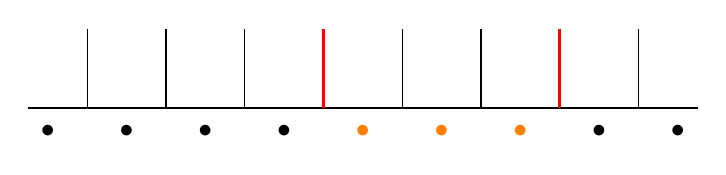
\begin{tikzpicture}
		\draw (-0.25,0) -- (8.25,0);
		\draw (0.5,0) -- (0.5,1);
		\draw (1.5,0) -- (1.5,1);
		\draw (2.5,0) -- (2.5,1);
		\draw[red,line width=0.4mm] (3.5,0) -- (3.5,1);
		\draw (4.5,0) -- (4.5,1);
		\draw (5.5,0) -- (5.5,1);
		\draw[red,line width=0.4mm] (6.5,0) -- (6.5,1);
		\draw (7.5,0) -- (7.5,1);
		\node at (0,-0.3) {$\bullet$};
		\node at (1,-0.3) {$\bullet$};
		\node at (2,-0.3) {$\bullet$};
		\node at (3,-0.3) {$\bullet$};
		\node at (4,-0.3) {{\color{orange}$\bullet$}};
		\node at (5,-0.3) {{\color{orange}$\bullet$}};
		\node at (6,-0.3) {{\color{orange}$\bullet$}};
		\node at (7,-0.3) {$\bullet$};
		\node at (8,-0.3) {$\bullet$};
		\end{tikzpicture}
	\end{figure}
\noindent
where the colour of the orange bullets is not determined by the labels on the boundary of the chain. Hence, we get an additional qubit. In general, the number of additional qubits in the chain is $\#\mathrm{defects}-1$. This can be done analogously for the chain with periodic boundary conditions, the only difference is that in this case, we already have one qubit when there is no defect.

We could also allow the bimodule object to live on the horizontal lines of the chain. In particular,
We now want to build a chain out of $\Vec(\Z/2\Z)$ and the bimodule $F_1$ in the following way: consider the chain
\begin{figure}[H]
	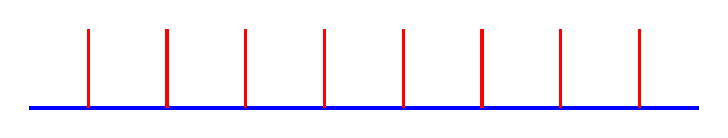
\begin{tikzpicture}
	\draw[blue,line width=0.4mm] (-0.25,0) -- (8.25,0);
	\draw[red,line width=0.4mm] (0.5,0) -- (0.5,1);
	\draw[red,line width=0.4mm] (1.5,0) -- (1.5,1);
	\draw[red,line width=0.4mm] (2.5,0) -- (2.5,1);
	\draw[red,line width=0.4mm] (3.5,0) -- (3.5,1);
	\draw[red,line width=0.4mm] (4.5,0) -- (4.5,1);
	\draw[red,line width=0.4mm] (5.5,0) -- (5.5,1);
	\draw[red,line width=0.4mm] (6.5,0) -- (6.5,1);
	\draw[red,line width=0.4mm] (7.5,0) -- (7.5,1);
	\end{tikzpicture}
\end{figure}
\noindent
where
\begin{equation}
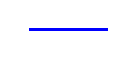
\begin{tikzpicture}[scale=1,baseline=(current bounding box.center)]
\draw[blue,line width=0.4mm] (0,0) -- (1,0);
\end{tikzpicture}=
\begin{tikzpicture}[scale=1,baseline=(current bounding box.center)]
\draw[black] (0,0) -- (1,0);
\end{tikzpicture}\oplus
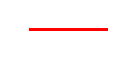
\begin{tikzpicture}[scale=1,baseline=(current bounding box.center)]
\draw[red,line width=0.4mm] (0,0) -- (1,0);
\end{tikzpicture},
\end{equation}
which means that it is either an object from the category ($0$ or $1$) or an object from the bimodule (which can only be $*$), i.e., $\mathbb{C}^2\oplus\mathbb{C}\cong\mathbb{C}^3$. Valid configurations then look like
\begin{figure}[H]
	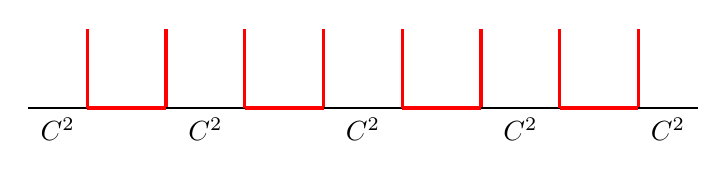
\begin{tikzpicture}
	\draw[black] (-0.25,0) to node [below] {$\mathbb{C}^2$} (0.5,0);
	\draw[red,line width=0.4mm] (0.5,0) -- (0.5,1);
	\draw[red,line width=0.4mm] (0.5,0) -- (1.5,0);
	\draw[red,line width=0.4mm] (1.5,0) -- (1.5,1);
	\draw[black] (1.5,0) to node [below] {$\mathbb{C}^2$} (2.5,0);
	\draw[red,line width=0.4mm] (2.5,0) -- (2.5,1);
	\draw[red,line width=0.4mm] (2.5,0) -- (3.5,0);
	\draw[red,line width=0.4mm] (3.5,0) -- (3.5,1);
	\draw[black] (3.5,0) to node [below] {$\mathbb{C}^2$} (4.5,0);
	\draw[red,line width=0.4mm] (4.5,0) -- (4.5,1);
	\draw[red,line width=0.4mm] (4.5,0) -- (5.5,0);
	\draw[red,line width=0.4mm] (5.5,0) -- (5.5,1);
	\draw[black] (5.5,0) to node [below] {$\mathbb{C}^2$} (6.5,0);
	\draw[red,line width=0.4mm] (6.5,0) -- (6.5,1);
	\draw[red,line width=0.4mm] (6.5,0) -- (7.5,0);
	\draw[red,line width=0.4mm] (7.5,0) -- (7.5,1);
	\draw[black] (7.5,0) to node [below] {$\mathbb{C}^2$} (8.25,0);
	\end{tikzpicture}
\end{figure}
\noindent
so we have a non-trivial Hilbert space. We will now construct a Hamiltonian for this chain that is similar to the golden chain Hamiltonian in \cite{Feiguin2007}, where a chain model for the Fibonacci category was constructed which energetically favoured fusing to the vacuum. For our chain model, this means that it is energetically favoured to fuse to the $0$ object of $\Vec(\Z/2\Z)$. Hence, the Hamiltonian is of the form
\begin{equation}
H=-\sum \frac{1}{\sqrt{2}}
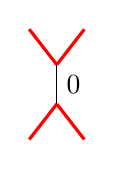
\begin{tikzpicture}[scale=0.5,baseline=(current bounding box.center)]
\draw[red,line width=0.4mm] (0,0) -- (-0.7,0.9);
\draw[red,line width=0.4mm] (0,0) -- (0.7,0.9);
\draw (0,0) to node[right] {$0$} (0,-1);
\draw[red,line width=0.4mm] (0,-1) -- (-0.7,-1.9);
\draw[red,line width=0.4mm] (0,-1) -- (0.7,-1.9);
%			\node at (0.8,1.1) {$*$};
%			\node at (-0.8,1.1) {$*$};
%			\node at (0.8,-2.1) {$*$};
%			\node at (-0.8,-2.1) {$*$};
\end{tikzpicture},\label{VecZ2Hamiltonian}
\end{equation}
where the sum goes over all sites of the chain. This Hamiltonian involves the vertex
\begin{figure}[H]	
	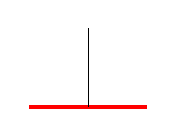
\begin{tikzpicture}
	\draw[red,line width=0.4mm] (0,0) -- (1.5,0);
	\draw[black] (0.75,0) -- (0.75,1);
	\end{tikzpicture}.
\end{figure}
\noindent
Since this vertex is neither defined in the category $\Vec(\Z/2\Z)$ nor in the bimodule $F_1$, we need to construct it. More precisely, for each choice of labels we need a basis for the corresponding morphism space. 
%For now, we will restrict to the case that only objects of the category are allowed to be on horizontal lines, but we will come back to other possibilities later. Although we will not need this specific vertex in the final chain we are going to construct, we go through its computation in detail to explain how these vertices can be constructed in general. 
We do the construction of the required vertex step-by-step in Section~\ref{Ising} using ideas from tube algebras. Therefore, we familiarize the reader with this concept first.